\chapter{Background \& Objectives}

% This section should discuss your preparation for the project, including background reading, your analysis of the problem and the process or method you have followed to help structure your work.  It is likely that you will reuse part of your outline project % specification, but at this point in the project you should have more to talk about. 

\section{Introduction}
The project aim was to create an application that could report on the quality of a metagenome assembly  provided by the user, presenting them with feedback about the contiguous reads contained in their data. The requirements for the project topic were very open, as there are multiple techniques for attempting to report the quality of a single species genome assembly, and while some can be used for metagenome assemblies, it was believed that no one tool covered this area yet with numerous techniques. Likewise, the way in which the results could be presented to the user was not established and open to my own interpretation.

%======= BACKGROUND ==========

\section{Background}
Before the project began, my knowledge of metagenomics was very limited, close to none. However, I liked the project title and description and thought it would be an interesting and challenging topic to learn new domain knowledge, use different technologies and attempt to implement an application where I had to learn from the ground up. On top of this, I find DNA to be an intriguing topic even with my limited knowledge and I was curious to learn more as I worked on this project.

My first step was trying to understand what exactly it was I was expected to produce at the end of the project. As the requirements of the resulting application were so open, it was up to me to research what metagenomics is, what is meant by `quality' within the subject, how this quality might be found and reported on, what technologies would be appropriate and what quality techniques could be used.

\subsection{Metagenomics}
Metagenomics is the study of environmental samples of genomic data where the contents of the data are potentially unknown and unclear. It has been described as `Open-ended sequencing of nucleic acids recovered directly from samples without culture or target-specific enrichment or amplification; usually applies to the study of microbial communities.'\cite{citeulike:14021056} It can be used in the findings of what an animal gut may contain, what viruses are within a sample when looking into outbreaks and finding what microbial communities exist in a sample area.

Metagenomics is a hot and interesting topic in the bioinformatics field, and its uses grow as more is learned, but there is the issue of quality, and how a metagenomic sample should be processed. To help me better understand the project task, I read articles that attempted to provided ways of analyzing metagenomic data to get the best quality results at the end.\cite{citeulike:11448654}

\subsection{Understanding Quality}

Considering the nature of metagenomics and the unknowns, it becomes clear quite quickly that when a sample you have is run through an assembler in an attempt to create a genome for sequencing, without the proper tools to quality assess your data you cannot be sure if what you are creating is an actual thing that could exist in nature. The process of taking a sample through to sequencing with metagenomic data can be very error prone, leading to misassemblies with duplicate or short reads, or combining reads together to make chimeric contiguous reads (contig).\cite{citeulike:3746363}

A chimieric contig is an instance where an assembler has put together reads from a sample that it believed were part of the same whole, and yet were in fact of different species/sub-species, and so creates a contig that does not actually exist in nature. It can be understood then that if a user were to sequence this, unless that is the result that they wanted, it won't be of any use to them. Without the proper tools, how would they know that their assembly data contains chimeric contigs and are not just wasting their time and money?

We can visualize this through  the diagram below, where we take a number of reads, put them through an assembler and the output is a number of contigs that the assembler believes it has created correctly, but may in fact be chimeric.

\begin{figure}[H]
	\centering
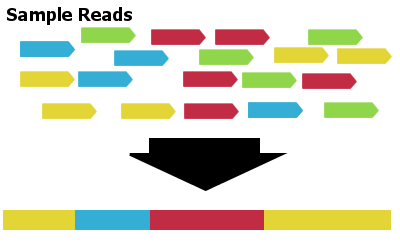
\includegraphics[width=0.5\textwidth]{images/basicmetaassembly}
	\caption{A very small example of a number of reads being taken into an assembler and the output of a contig where there may be a chimera.}
\end{figure}

If we imagine each of the colours representing an individual species (though in reality, there would be no colours, only the characters of data, and potentially hundred to thousands of different species and sub species in a sample) we could, by eye, see how we could extract some interesting genome data, for example taking all of the green in the order they are presented and finding the `green' genome. As naive as that is, it serves then to demonstrate that if we look at the output of the one contig shown in the figure, we can see how the  colours are aligned in a way that they are mixed.

It is possible that the resulting contig is a valid genome that could be found in nature, where the particular sequences in the different coloured sections are shared between each colour `species' and so this contig could work. However, it is also likely that the different coloured sections are widly different than the natural connecting colours if instead this contig was made up of a single colour (in this figure, all yellow, all blue, etc). This would then be a chimera. This demonstrates that without some quality assessment tools to attempt to report on where these misaligns have occurred, a user may never know if what they have is good quality data or not.

\subsection{Existing Software}
There are a number of tools I discovered in my background research that attempt to aid in the quality assessment of metagenomic data, in particular MEGAN, a `next-generation metagenomic data, called MEtaGenomeANalyzer', which attempts to do a taxonomical analysis comparison to known reference data\cite{citeulike:10457549} and PRINSEQ, a tool which provides `summary statistics of FASTA (and QUAL) or FASTQ files in tabular and graphical form'\cite{citeulike:8714996}.

The purpose of MEGAN is to look at user uploaded data sets and compare their data against numerous reference databases of known sequences, and then take the resuling comparison data and display it to the user in an interactive analysis visualisation. it uses a number of techniques to format the users data to check against the reference databases to maximize useful results. The aim of MEGAN is to try to determine what is in the sequences the user provides, if they exist already and how they compare to known reference datasets.

PRINSEQ is a web service (or standalone) tool written in Perl that lets users see statistical analysis data of their metagenome sequences through uploading FASTA files. It allows them to trim, filter and reformat their sequences, and a user can upload files of up to 600MB. Its aim is similar to the task set out for this project, in that it wishes to reduce the amount of time and money wasted on analyzing and interpreting poor metagenomic data.

When considering what my own application should do, I looked at the techniques used for PRINSEQ most, as these seemed to match up with what I thought would be useful to a user for my own application, and from discussing the topic with my supervisor I found techniques such as the GC Content distribution could be a good place to start.

It was not just tools for metagenomic quality assessment I looked into. I also found the NCBI database and their BLAST tool\cite{citeulike:11826724}, and kept in mind these may be useful as I progressed through my applications development.

BLAST (Basic Local Alignment Search Tool) allows user to search databases for different sequences and find regions of similarity between biological sequences. A user could upload their own sequence and have it aligned against known sequences to see if it already exists in the reference databases. This could be useful to be used in a metagenome quality toolkit, similar to MEGAN, through letting the user know that their assembly data has some similarities to existing sequences, which might indicate good quality.

Through reading an article that discussed the advantages of k-mer frequency analysis for quality assessment, I looked into the Jellyfish\cite{citeulike:8643499} and BFCounter\cite{citeulike:9639487} tools for just this role where I could potentially consume the output of their processing, although they took a step back in my mind while I considered what it was I actually wanted my application to be and worked out the requirements.

Jellyfish is a k-mer counting application that runs on the command line and uses the CPUs `compare and swap' function and encoding with a hash table to increase efficiency. On the other hand, BFCounter uses a Bloom Filter (a probabilistic data structure) to count k-mers, counting those k-mers that appear more than once and ignoring the singleton k-mers, as they are most likely not important to the data. Both take different methods for counting k-mers, and find their own ways for efficiency. If I wished to implement some kind of k-mer frequency analysis tool into my application, I would need to look into efficiently counting k-mers too.

%========== ANALYSIS =============

\section{Analysis}
After understanding the project topic and problem a little better, I decided upon a number of requirements of the application to begin with. Some of these were definite goals, some stretch goals and some future development tasks if I were to finish all else or were to continue the application after the project deadline. I broke the problem down into its two core components steps, the analysis and the report. I felt that the resulting list that can be seen below was enough to work with based on the knowledge I had gained from my background reading and what I thought would be appropriate for the time allotted for the project.

\subsection{Quality assessment}
The quality assessment had to use a number of methods suitable enough to produce some data or statistics that could indicate to the user a measure of quality of their assembly data. For this end, I decided upon a number of objectives:

\subsubsection{Contig length}
`Give the user control over the minimum length a contig should be to be considered.'

This measure would be good in displaying where an assembler could not find any reads to match with a single read and so didn't do anything more with it than output it as a contig of an individual read length. This would most likely indicate that it is of no use to a user, as a contig the size of a read length is unlikely to contain any useful genome data. Allowing a user to set the minimum length threshold lets them set their own size, be it the known read length size of their data, or a size they think would be appropriate to start seeing some usable data from contigs with length over a particular amount/number of read lengths.

\subsubsection{Number of unknown characters}
`The application should count the number of unknown (N) characters within a contig.'

When an assembler cannot understand what to do with a character, or a sequence of characters, it may insert an `N' character. Indicating to a user how many of these exist in a contig, and what percentage of the whole they make up is a helpful indication of whether their data is of good quality or not, with the less or no unknowns the better the quality.

\subsubsection{GC Content}
`Conduct a GC Content percentage analysis in sliding windows of a size set by the user.'

The GC content is the percentage of `G' (guanine) and `C' (cytosine) characters within a sequence\cite{citeulike:14021291}. When the application takes a contig, it should break the contig up into windows of a size set by the user. If a contig was of length 30,000, they might break it into 100 windows of 300, for example. These window sizes should then have their GC content percentage calculated, and the mean of the entire contigs GC content worked out. Using these values it then becomes possible to detect potential anomalies in the percentages of individual windows that have a percentage value drastically different than the mean.

\subsubsection{Open Reading Frame Locations}
`To confirm if a GC window is outside of the mean by misalign, Open Reading Frame (ORF) Locations should be found where the GC content would naturally be higher in protein coding regions.'

This addition to the requirements came later in the projects development as I came to understand GC content and how a window that looks like an area of a misalign may actually not be. We can look at a contiguous read and find protein coding regions through the use of Open Reading Frames\cite{orfdefinition}, where the GC content percentage is often naturally higher than outside of these regions.\cite{JEU:JEU239}

An ORF Location is found through looking for where a location starts with ATG and where it ends with TGA, TAA or TAG. There are 6 frames to be found in sequences, where three are `forward' and 3 are `backwards' with the opposite characters of the base pairs to the forward frames. For both forward and backwards, the first frame is the original sequence, the second frame begins one character into the sequences and the third frame begins two characters into the sequence. A very small example just for basic understanding is provided below:

\begin{verbatim}
Sequence:
TTGATGGCGCATAG

Frame \#1 (fwd):
TTGATGGCGCATAG
Frame \#2 (fwd):
TGATGGCGCATAG
Frame \#3 (fwd):
GATGGCGCATAG
Frame \#4 (bck):
CTATGCGCCATCAA
Frame \#5 (bck):
TATGCGCCATCAA
Frame \#6 (bck):
ATGCGCCATCAA
\end{verbatim}

By finding the ORF Locations, we can use these in the quality report to match up to windows that may at first seem like anomalies in the contig where it is instead actually a natural occurrence. There is a preexisting tool for this ORF finding functionality by NCBI\cite{orffinder}. While it might not be the case that an ORF Location matches with an out of threshold GC content window, or that they do match but it is still in fact an anomaly, it was a requirement of the application I wished to include in order to give the user another tool to use for inspecting their data.

\subsubsection{K-mer frequency analysis}
`The application should conduct a k-mer frequency analysis, or use output of k-mer frequency analysis tools.'

Conducting k-mer frequency analysis in window sizes has a similar output as GC content, except we look for the frequency of particular `k-mer' (where `k' is a number of how many characters to be considered, e.g. 3mer `ATG', 4mer `ATGA'). Through measuring the frequency in windows we could see if there was an even distribution of frequencies across a contig, and if any windows had large changes in the frequencies that could indicate a potentially bad quality contig.\cite{citeulike:12566531}

This was set as a stretch requirement, as the process of efficiently conducting k-mer frequency analysis and the research into the possibility of writing my own software to do it or consuming output of another application was expected to take over the time for the project, after my background reading and understanding was completed and the other features previously mentioned implemented.

\subsubsection{NCBI reference data}
`The application should compare the contiguous read data to known reference data in the NCBI database with BLAST.'

Using the known reference data, much like with MEGAN, it would be possible to see if any of the contigs in the user data match to known reference data and so can be considered good quality. This was a stretch requirement though, with the idea more in mind for if the application were to be continued to be developed after the project deadline.

\subsection{Quality report and data input}
\subsubsection{Read user input in FASTA format}
`A user should be able to paste or upload their data in FASTA format.'

The FASTA format is a commonly used format for sequence data. It is `a text-based format for representing either nucleotide sequences or peptide sequences' \cite{fastaformat}. It is formatted in the way that can be seen in the figure below. I set myself the task for allowing the upload and paste of data, beginning with pasting the data into a form, as uploading data could add a larger realm of security and data size issues and so I wanted to have the simplest thing possible first.

\begin{figure}[H]
\centering
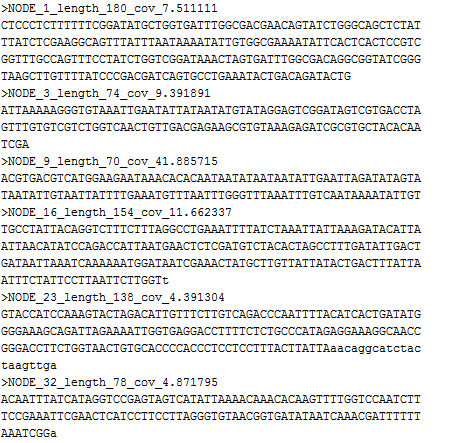
\includegraphics[width=0.5\textwidth]{images/fastaexample}
\caption{A small example of the contents of a FASTA file, with very short contigs. The example is just to show the format of how multiple contiguous reads are stored in the same FASTA file.}
\end{figure}

For the FASTA format my application accepted, I planned for it to begin only taking into account ATGC \& N as characters to deal with, where N was `unknown/unclear' and the other characters were valid. Uppercase and lowercase characters would be preserved in any output display of the application, but capitalization would not taken into account for any of the processes as they did not make a difference to the quality assessment techniques.

\subsubsection{Display a list of the contigs}
`A user should be able to see the contiguous reads listed in their FASTA data.'

I decided it would be a good idea to display to the user the list of contigs that their file contained, with small bits of relevant information, such as the size of the contig, the header of it and the previously mentioned `N' count and percentage. From here a user would be able to select a contig they wish to further inspect for quality issues.

\subsubsection{User control over GC Content, ORF Location and k-mer frequency analysis parameters}
`When conducting a quality inspection, a user should be able to adjust the parameters of the methods based upon their expectations, data input and choice.'

Since the data uploaded by a user would have been assembled from reads of a particular length, the appropriate size of GC content and k-mer frequency windows, minimum size of ORF Location lengths and minimum length of contigs should be set by the user. It could have been a possibility to guess what a good size would be for the user (i.e. find the shorted contig in the data and consider that that might be the size of a single read, and suggest length parameters based on that).

\subsubsection{Visual reports of the quality inspection methods}
`A user should be able to see a visual representation of a contigs GC content and any anomalies.'

In order for a user to be shown whether their data is of good quality or not, visualizations would be required that highlight any problem areas, or if areas are not highlighted, at least give them a broad sense of the layout of the results of the quality inspection to allow them to analyze the results from themselves. This should include displays for GC content in windows, ORF Locations broken into individual frames, k-mer frequency analysis in windows and a comparison shown between the GC content and ORF Locations.

I did consider how I could potentially provided a quality confidence factor to a user, or how I might demonstrate to them in a statistical way that their data was of good or bad quality. However, with the amount of methods that could be used, the unclarity of the data itself and the users expectations, I felt that it would be better to instead provide the user with visuals to analyze the results of my application themselves, and I would instead try to highlight problem areas without necessarily saying clearly `This is/is not a problem area'.

\begin{figure}[H]
 \centering
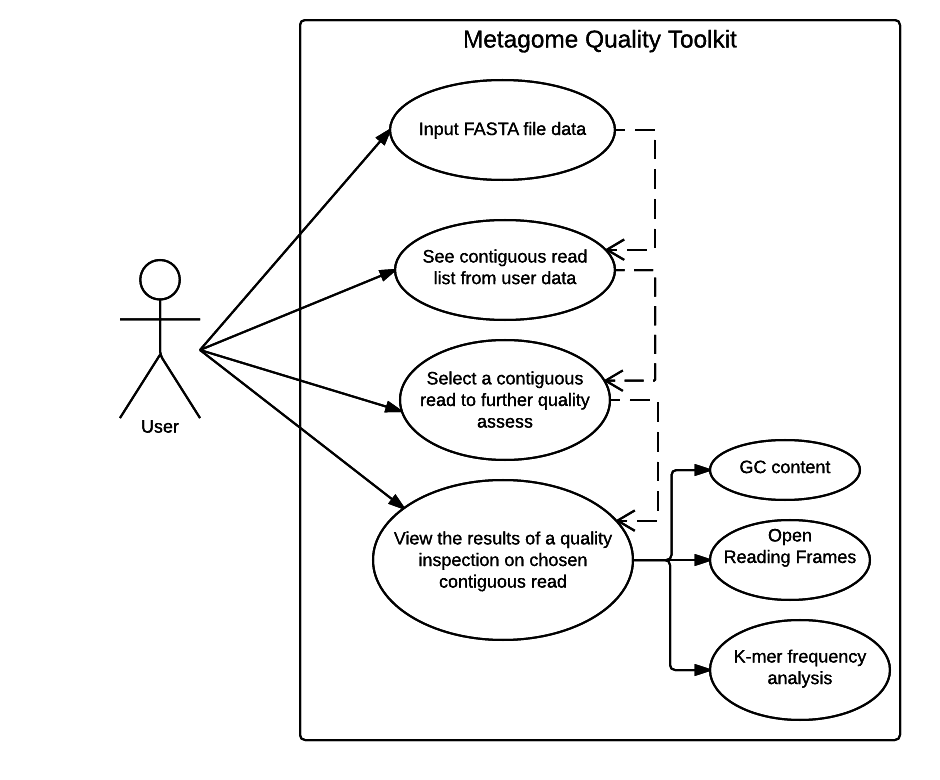
\includegraphics[width=0.9\textwidth]{images/usecase}
\caption{A use case diagram demonstrating the expected functionality for a user based on the functional requirements laid out in this section.}
\end{figure}

\subsection{Implementation - 3rd Party vs Self-Created}
Based on the requirements I had selected, I decided that I wanted to write my own software for each functional component. While solutions for each component exists individually, I felt there would be more benefit to a user if I could produce my own software to support the functionality, over requiring them to use third part software in order to use my application too.

Additionally to this, I wanted the technical challenge of writing my own software, and enabling the application to be maintainable and expanded upon in the future rather than relying on third party support applications in order to process a users input. The process of developing the application from scratch would also give me the opportunity to learn more about the domain and technologies for development than just consuming output of other existing applications, even if achieving the end result would take more time.

While I knew the project would come to a close on development at the end of the semester, I also wanted to envision this as a project that could be taken forward in the future to be further developed and maintained. For this reason it also made sense to develop my own application without consuming output from third party software, excluding the FASTA files from an assembler. If one of these third party applications was no longer available or their output changed, it would render my application unusable or require more future modification to adapt to changes by outside sources.

%======== PROCESS ==========

\section{Process}
An agile methodology seemed most appropriate for this project development, due to the unclear requirements (based on my lack of understanding and the open tasks at the start of the project) and would allow me to break down each requirements into stories, and then into tasks and get a thin slice of the application done quickly, and build outwards from there, always ensuring I had some finished product at each functional completion. While my project could well follow a plan driven approach, such as waterfall or the spiral model, I believed that an agile approach would be more suitable for developing it. 

I chose to use Scrum for my framework, and used aspect of Extreme Programming for my daily development cycle, adapted to a one person project. Considering the  nature of my projects requirements, I considered if I should instead use Feature Driven Development, but decided upon Scrum due to my experience with it through my industrial year and in that I could see how I could break the requirements down in to user stories and tasks.

\subsection{Scrum}
Scrum is an agile framework for developing complex products\cite{Schw01a}. In brief, it works in iterations (Sprints) where work is broken into user stories and tasks for those stories, there are key members of the team who have designated roles (Engineer, QA, Scrum Master, Product Owner, etc) and where each Sprint has meetings involved in it to help the flow of work: Sprint Planning \& Sprint Retrospectives, Sprint Review and Daily Stand-ups. I decided that adopting this framework would help me structure my weekly work and aid me in planning and development for the project.

As a one-person project, a number of the components of Scrum either had to be dropped or adapted, for example, the roles of team members were all adopted by myself rather than having actual team members. I worked on a weekly Sprint cycle, where at the beginning of every Tuesday a new Sprint would begin, and I would review the work done and have a Retrospective with myself and plan out the next weeks tasks, often through talking with my supervisor. As for Daily Stand-ups, I was able to carry these out through holding them with my peers, Alex Jollands and Sion Griffiths. Between the three of us we would meet in-person or using Internet calls on weekday mornings at 10am and discuss our work from the day before, the planned work for the current day and anything we wanted to soundboard off one another.

The Scrum framework had me taking my initial planned out requirements and turn them into Stories with their own tasks. Stories are structured in the way of:
\newline

`As a \textless \textit{type of user}\textgreater, I want \textless \textit{some goal}\textgreater so that \textless \textit{some reason}\textgreater.'\cite{userstories}
\newline

Once a user story has been created, I would then consider it and see if I could break it down into a `narrow slice'; the simplest, thinnest possible thing I could do for a feature implementation that would produce results. There is an example of this in Appendix 3 `Examples and Extras' under `Example User Story Breakdown'. Breaking down the requirements into user stories and then tasks helped me focus on what was important, and gauge what needed to be done and how much effort vs time it would take.

\subsection{Extreme Programming}
For the day to day development outside of the Scrum framework, I decided to adopt a modified Extreme Programming (XP) approach\cite{xp}. While I couldn't do all of the XP techniques (pair programming, for example), I strongly took the elements of Test Driven Development (TDD), refactoring, simple design (coding only what needs to be done based on the TDD and refactoring) and continuous integration. I felt that using a combination of Scrum and XP techniques was a suitable process for my application, and would aid me in my design, implementation, testing, meeting the requirements and focusing my motivation.

The motivation for taking the aspects of TDD and Refactoring were that I could build and design my application iteratively, as I understood and refined the requirements and functionality of the application as I went, while still having a usable application from an early stage that could be developed upon in each Sprint. This helped me in having an evolving design for the application, while not having a design document but still laying out the structure of the application to a good standard.

TDD ensured that the application would be developed in the simplest way possible, and always meet the requirements currently tested for by doing the unit test development up front. Refactoring the work as I went and where needed meant that I would keep my code maintainable while developing in this way. The end result through selecting this methodology was to aim for a robust, maintainable, well-design application with test coverage for all functionality and programmed efficiently through proper time management.

Using continuous integration meant that I could be sure that whenever I completed a new bit of code, it would be run against all existing tests to check that nothing had broken and was impacting previously working functionality.

\subsection{Pomodoro Technique}
On the matter of time management during development time, I found it useful to break my work into small cycles using the Pomodoro technique\cite{citeulike:14021988} to increase my focus and productivity. The aim of the Pomodoro technique is to spend 25 minutes with full focus on the work, and then spend 5 minutes to stop and have a break. They are also useful for keeping track of work done and visually seeing how much time has been invested into the project for the day. To record my pomodoros I used \url{http://www.tomato.es/}.
 
Due to the short length of each pomodoro, it was also seen as an effective method for squeezing in work where there was time. By quantifying time into small slots, it made it possible to consider how much time I might have between other events in the day and work out where it could be possible to put in a single pomodoros worth of work. This is instead of perhaps not working because I felt I did not have the time, or working and eating into other daily activities if I didn't block out the time and be aware of when to stop.

\subsection{Project blog}
While developing my application I kept a blog about my project, any milestones I reached or interesting sections. While I did not designate a particular time to blog, I believed it would be a useful tool in reflecting on the work done when writing this report, something for my supervisor to be able to check upon my progress between meetings and give me the time to reflect on the work done and any upcoming tasks to help me mentally process where the project was in its life cycle against the planned objects. The blog may be seen at \url{http://users.aber.ac.uk/jee22/wordpress/}.
